

\documentclass[landscape,final,a0paper,fontscale=0.285]{baposter}
    \renewcommand{\refname}{}
\usepackage{calc}
\usepackage{graphicx}
\usepackage{epstopdf}
\usepackage{amsmath}
\usepackage{amssymb}
\usepackage{relsize}
\usepackage{multirow}
\usepackage{rotating}
\usepackage{bm}
\usepackage{url}
\usepackage{cite}
\usepackage{graphicx}
\usepackage{multicol}

%\usepackage{times}
%\usepackage{helvet}
%\usepackage{bookman}
\usepackage{palatino}



\newcommand{\captionfont}{\footnotesize}

\graphicspath{{images/}{../images/}}
\usetikzlibrary{calc}

\newcommand{\SET}[1]  {\ensuremath{\mathcal{#1}}}
\newcommand{\MAT}[1]  {\ensuremath{\boldsymbol{#1}}}
\newcommand{\VEC}[1]  {\ensuremath{\boldsymbol{#1}}}
\newcommand{\Video}{\SET{V}}
\newcommand{\video}{\VEC{f}}
\newcommand{\track}{x}
\newcommand{\Track}{\SET T}
\newcommand{\LMs}{\SET L}
\newcommand{\lm}{l}
\newcommand{\PosE}{\SET P}
\newcommand{\posE}{\VEC p}
\newcommand{\negE}{\VEC n}
\newcommand{\NegE}{\SET N}
\newcommand{\Occluded}{\SET O}
\newcommand{\occluded}{o}


%%%%%%%%%%%%%%%%%%%%%%%%%%%%%%%%%%%%%%%%%%%%%%%%%%%%%%%%%%%%%%%%%%%%%%%%%%%%%%%%
%%%% Some math symbols used in the text
%%%%%%%%%%%%%%%%%%%%%%%%%%%%%%%%%%%%%%%%%%%%%%%%%%%%%%%%%%%%%%%%%%%%%%%%%%%%%%%%

%%%%%%%%%%%%%%%%%%%%%%%%%%%%%%%%%%%%%%%%%%%%%%%%%%%%%%%%%%%%%%%%%%%%%%%%%%%%%%%%
% Multicol Settings/
%%%%%%%%%%%%%%%%%%%%%%%%%%%%%%%%%%%%%%%%%%%%%%%%%%%%%%%%%%%%%%%%%%%%%%%%%%%%%%%%
\setlength{\columnsep}{1.5em}
\setlength{\columnseprule}{0mm}

%%%%%%%%%%%%%%%%%%%%%%%%%%%%%%%%%%%%%%%%%%%%%%%%%%%%%%%%%%%%%%%%%%%%%%%%%%%%%%%%
% Save space in lists. Use this after the opening of the list
%%%%%%%%%%%%%%%%%%%%%%%%%%%%%%%%%%%%%%%%%%%%%%%%%%%%%%%%%%%%%%%%%%%%%%%%%%%%%%%%
\newcommand{\compresslist}{%
\setlength{\itemsep}{1pt}%
\setlength{\parskip}{0pt}%
\setlength{\parsep}{0pt}%
}

%%%%%%%%%%%%%%%%%%%%%%%%%%%%%%%%%%%%%%%%%%%%%%%%%%%%%%%%%%%%%%%%%%%%%%%%%%%%%%
%%% Begin of Document
%%%%%%%%%%%%%%%%%%%%%%%%%%%%%%%%%%%%%%%%%%%%%%%%%%%%%%%%%%%%%%%%%%%%%%%%%%%%%%

\begin{document}

%%%%%%%%%%%%%%%%%%%%%%%%%%%%%%%%%%%%%%%%%%%%%%%%%%%%%%%%%%%%%%%%%%%%%%%%%%%%%%
%%% Here starts the poster
%%%---------------------------------------------------------------------------
%%% Format it to your taste with the options
%%%%%%%%%%%%%%%%%%%%%%%%%%%%%%%%%%%%%%%%%%%%%%%%%%%%%%%%%%%%%%%%%%%%%%%%%%%%%%
% Define some colors

%\definecolor{lightblue}{cmyk}{0.83,0.24,0,0.12}
\definecolor{lightblue}{rgb}{0.145,0.6666,1}

% Draw a video
\newlength{\FSZ}
\newcommand{\drawvideo}[3]{% [0 0.25 0.5 0.75 1 1.25 1.5]
   \noindent\pgfmathsetlength{\FSZ}{\linewidth/#2}
   \begin{tikzpicture}[outer sep=0pt,inner sep=0pt,x=\FSZ,y=\FSZ]
   \draw[color=lightblue!50!black] (0,0) node[outer sep=0pt,inner sep=0pt,text width=\linewidth,minimum height=0] (video) {\noindent#3};
   \path [fill=lightblue!50!black,line width=0pt] 
     (video.north west) rectangle ([yshift=\FSZ] video.north east) 
    \foreach \x in {1,2,...,#2} {
      {[rounded corners=0.6] ($(video.north west)+(-0.7,0.8)+(\x,0)$) rectangle +(0.4,-0.6)}
    }
;
   \path [fill=lightblue!50!black,line width=0pt] 
     ([yshift=-1\FSZ] video.south west) rectangle (video.south east) 
    \foreach \x in {1,2,...,#2} {
      {[rounded corners=0.6] ($(video.south west)+(-0.7,-0.2)+(\x,0)$) rectangle +(0.4,-0.6)}
    }
;
   \foreach \x in {1,...,#1} {
     \draw[color=lightblue!50!black] ([xshift=\x\linewidth/#1] video.north west) -- ([xshift=\x\linewidth/#1] video.south west);
   }
   \foreach \x in {0,#1} {
     \draw[color=lightblue!50!black] ([xshift=\x\linewidth/#1,yshift=1\FSZ] video.north west) -- ([xshift=\x\linewidth/#1,yshift=-1\FSZ] video.south west);
   }
   \end{tikzpicture}
}

\hyphenation{resolution occlusions}
%%
\begin{poster}%
  % Poster Options
  {
  % Show grid to help with alignment
  grid=false,
  % Column spacing
  colspacing=1em,
  % Color style
  bgColorOne=white,
  bgColorTwo=white,
  borderColor=lightblue,
  headerColorOne=black,
  headerColorTwo=lightblue,
  headerFontColor=white,
  boxColorOne=white,
  boxColorTwo=lightblue,
  % Format of textbox
  textborder=roundedleft,
  % Format of text header
  eyecatcher=true,
  headerborder=closed,
  headerheight=0.1\textheight,
%  textfont=\sc, An example of changing the text font
  headershape=roundedright,
  headershade=shadelr,
  headerfont=\Large\bf\textsc, %Sans Serif
  textfont={\setlength{\parindent}{1.5em}},
  boxshade=plain,
%  background=shade-tb,
  background=plain,
  linewidth=2pt
  }
  % Eye Catcher
  {
\includegraphics[height=5em]{img/lgpsealm.eps}}
  % 
  {\bf\textsc{Web Interface for daylighting design and feedback }\vspace{0.5em}}
  % Authors
  {\textsc{\{ Max Espinoza, Rebecca Nordhauser, Joshua Nasman, and Barbara Cutler \}}}
  % University logo
  {% The makebox allows the  to flow into the logo, this is a hack because of the L shaped logo.
    
\includegraphics[height=5.0em]{img/logo_cs_design_1.png}
  }

%%%%%%%%%%%%%%%%%%%%%%%%%%%%%%%%%%%%%%%%%%%%%%%%%%%%%%%%%%%%%%%%%%%%%%%%%%%%%%
%%% Now define the boxes that make up the poster
%%%---------------------------------------------------------------------------
%%% Each box has a name and can be placed absolutely or relatively.
%%% The only inconvenience is that you can only specify a relative position 
%%% towards an already declared box. So if you have a box attached to the 
%%% bottom, one to the top and a third one which should be in between, you 
%%% have to specify the top and bottom boxes before you specify the middle 
%%% box.
%%%%%%%%%%%%%%%%%%%%%%%%%%%%%%%%%%%%%%%%%%%%%%%%%%%%%%%%%%%%%%%%%%%%%%%%%%%%%%
    %
    % A coloured circle useful as a bullet with an adjustably strong filling
    \newcommand{\colouredcircle}{%
      \tikz{\useasboundingbox (-0.2em,-0.32em) rectangle(0.2em,0.32em); \draw[draw=black,fill=lightblue,line width=0.03em] (0,0) circle(0.18em);}}

%%%%%%%%%%%%%%%%%%%%%%%%%%%%%%%%%%%%%%%%%%%%%%%%%%%%%%%%%%%%%%%%%%%%%%%%%%%%%%
  \headerbox{Motivation}{name=problem,column=0,row=0}{
%%%%%%%%%%%%%%%%%%%%%%%%%%%%%%%%%%%%%%%%%%%%%%%%%%%%%%%%%%%%%%%%%%%%%%%%%%%%%%


  %Images for this section
  %{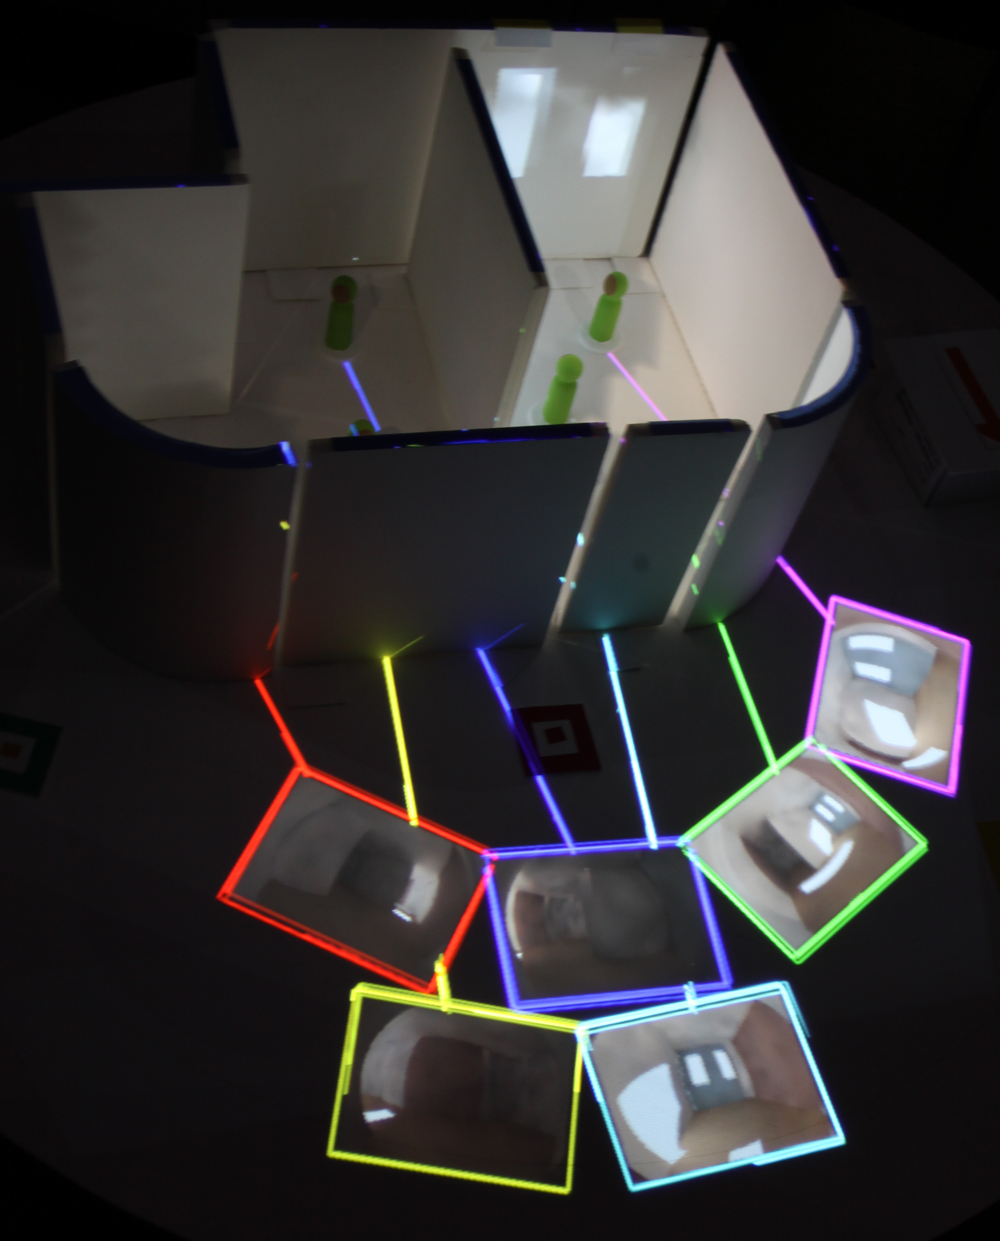
\includegraphics[height=10em]{img/office_color.jpg}}
  {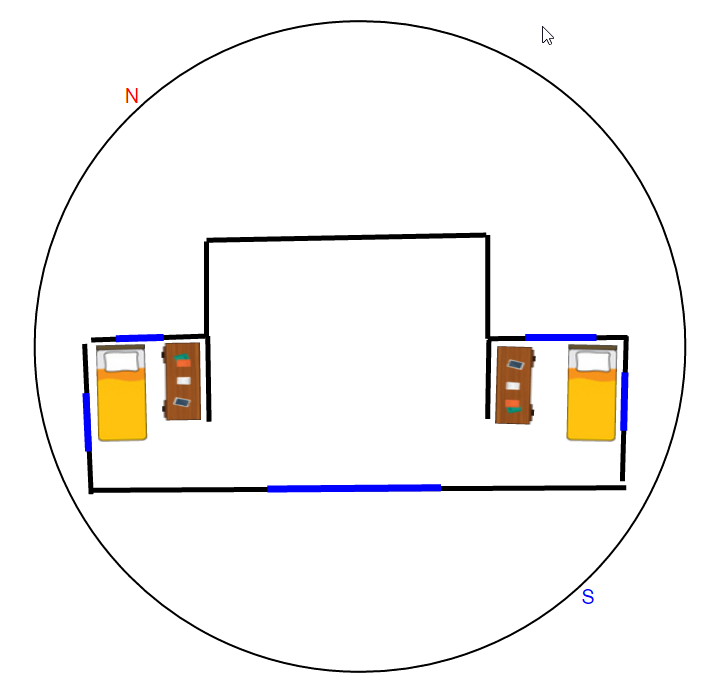
\includegraphics[height=10.25em]{img/oasis_1.png}}

  {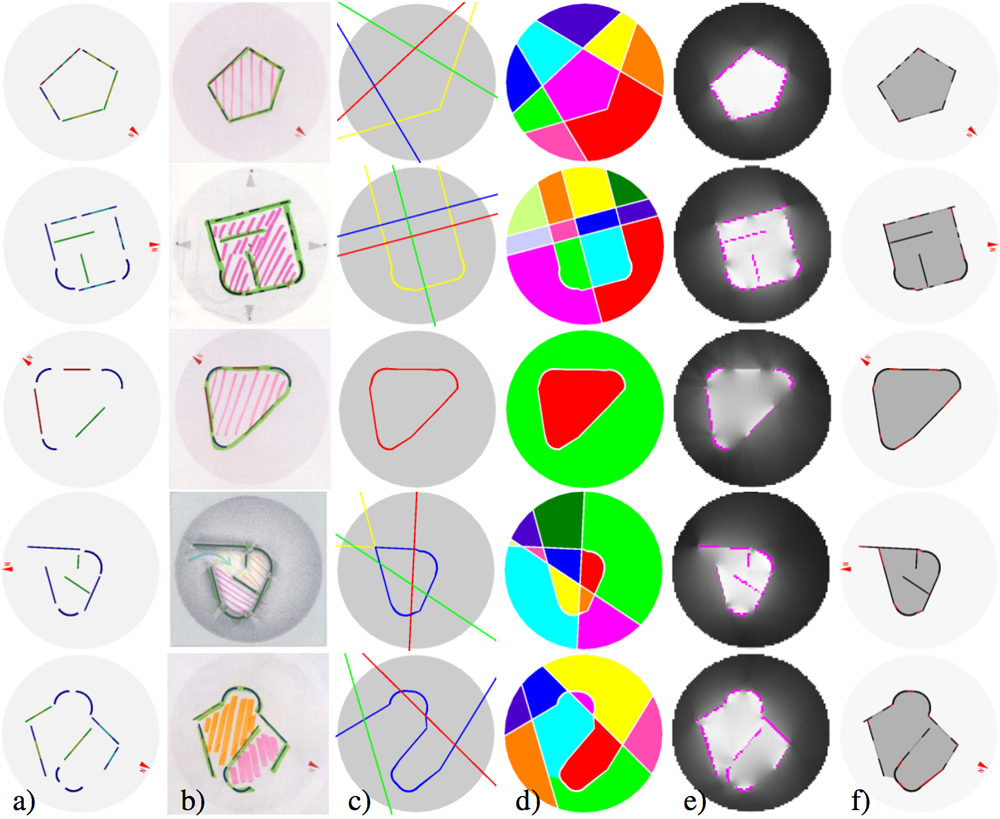
\includegraphics[height=13em]{img/aag_figure_3.png}}


  {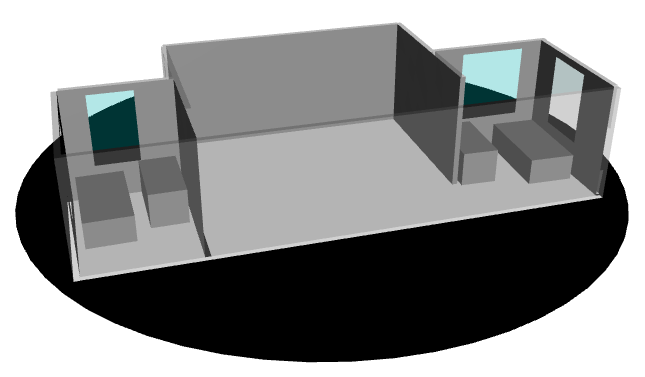
\includegraphics[height=10.25em]{img/oasis_2.png}} 
  %{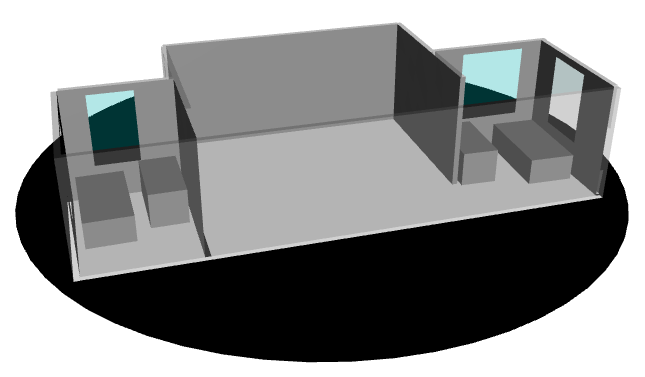
\includegraphics[height=11.25em]{img/oasis_2.png}}

  %text for this section
Previous research on the development of a spatially augmented tangible user interface for architectural daylighting simulation and design offered architects a novel approach in collaborative room design. \cite{NasmanEvaluation, ShengYYC09 }

User studies found the tools very helpful for visualizing lighting simulations and offered visual feedback to make better use of natural daylighting. Evaluation from this study lead to extending the interface to include avatars, illumination visualizations, and additional window models.\cite{NasmanEvaluation}

In order to collect more data we implemented an online interface which deliverers a set of capabilities similar to the physical system. Users are able to sketch designs which are translated into 3D models. Daylight simulated on these models relates illumination values to real world measurements.

 }%end section


%%%%%%%%%%%%%%%%%%%%%%%%%%%%%%%%%%%%%%%%%%%%%%%%%%%%%%%%%%%%%%%%%%%%%%%%%%%%%%
\headerbox{User Interface and Interactive Feedback}{name=userinterface,span = 2,column=2,,row=0}{
  %%%%%%%%%%%%%%%%%%%%%%%%%%%%%%%%%%%%%%%%%%%%%%%%%%%%%%%%%%%%%%%%%%%%%%%%%%%%%%
  {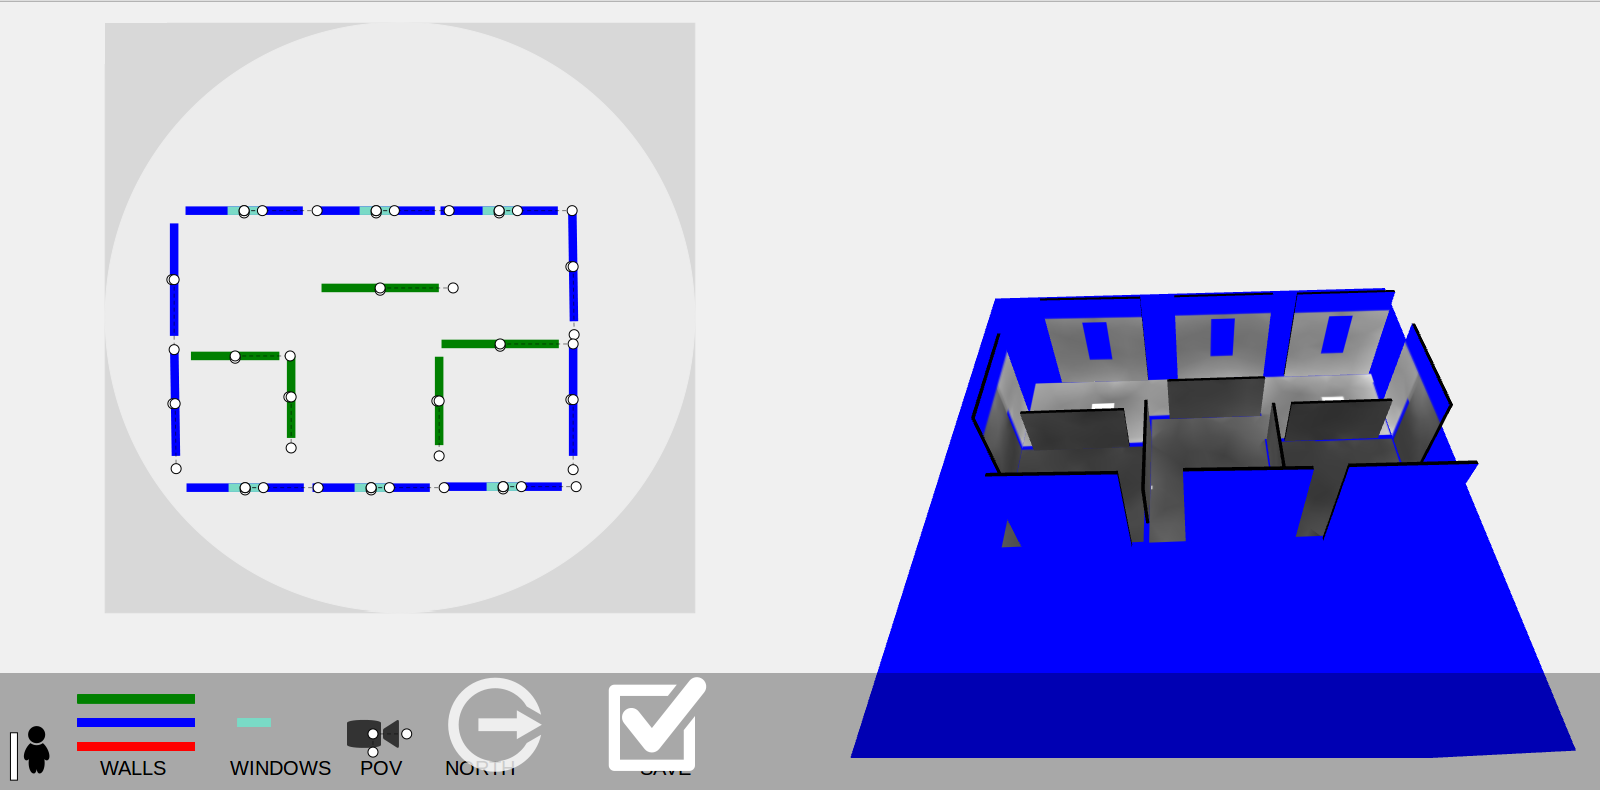
\includegraphics[width=42em]{img/combined.png}}
  
  \begin{multicols}{2}
  	\textbf{User Interface:} The interface offers a variety of tools to design and create floor layouts including wall selection, window placement, avatar points-of-view, and compass orientation.
  	
  	\textbf{Interactive Feedback:} After a design is saved, a 3D model of the floor plan renders on the right pane. This rendering is interactive such that can navigate around the model to view lighting from different view points. This view provides feedback which then the user can use alter their model to optimize natural daylighting usage. Moreover lighting visualization incorporated into these view points through avatar tokens can help users better understand illumintation in the 3D models.
  \end{multicols}
  \vspace{-0.6em}
   

}

%%%%%%%%%%%%%%%%%%%%%%%%%%%%%%%%%%%%%%%%%%%%%%%%%%%%%%%%%%%%%%%%%%%%%%%%%%%%%%
  \headerbox{Contributions}{name=contribution,column=1,row=0}{
%%%%%%%%%%%%%%%%%%%%%%%%%%%%%%%%%%%%%%%%%%%%%%%%%%%%%%%%%%%%%%%%%%%%%%%%%%%%%%
  
   Currently a working prototype of the application offers functionality similar to the physical system.
   We used WebGL and the Raphael graphics libraries to build both the user interface and 3D visualization. Our online application implements the following features.
   \begin{enumerate}\compresslist
   \item A simple drag and drop interface to design models with wall primitives
   %\item Avatar primitives that render geometry to view a POV scene
   \item Save and load user created layouts
   \item Interactive feedback that allows navigation through user generated spaces with simulated daylight
   \end{enumerate}
   
\begin{center}{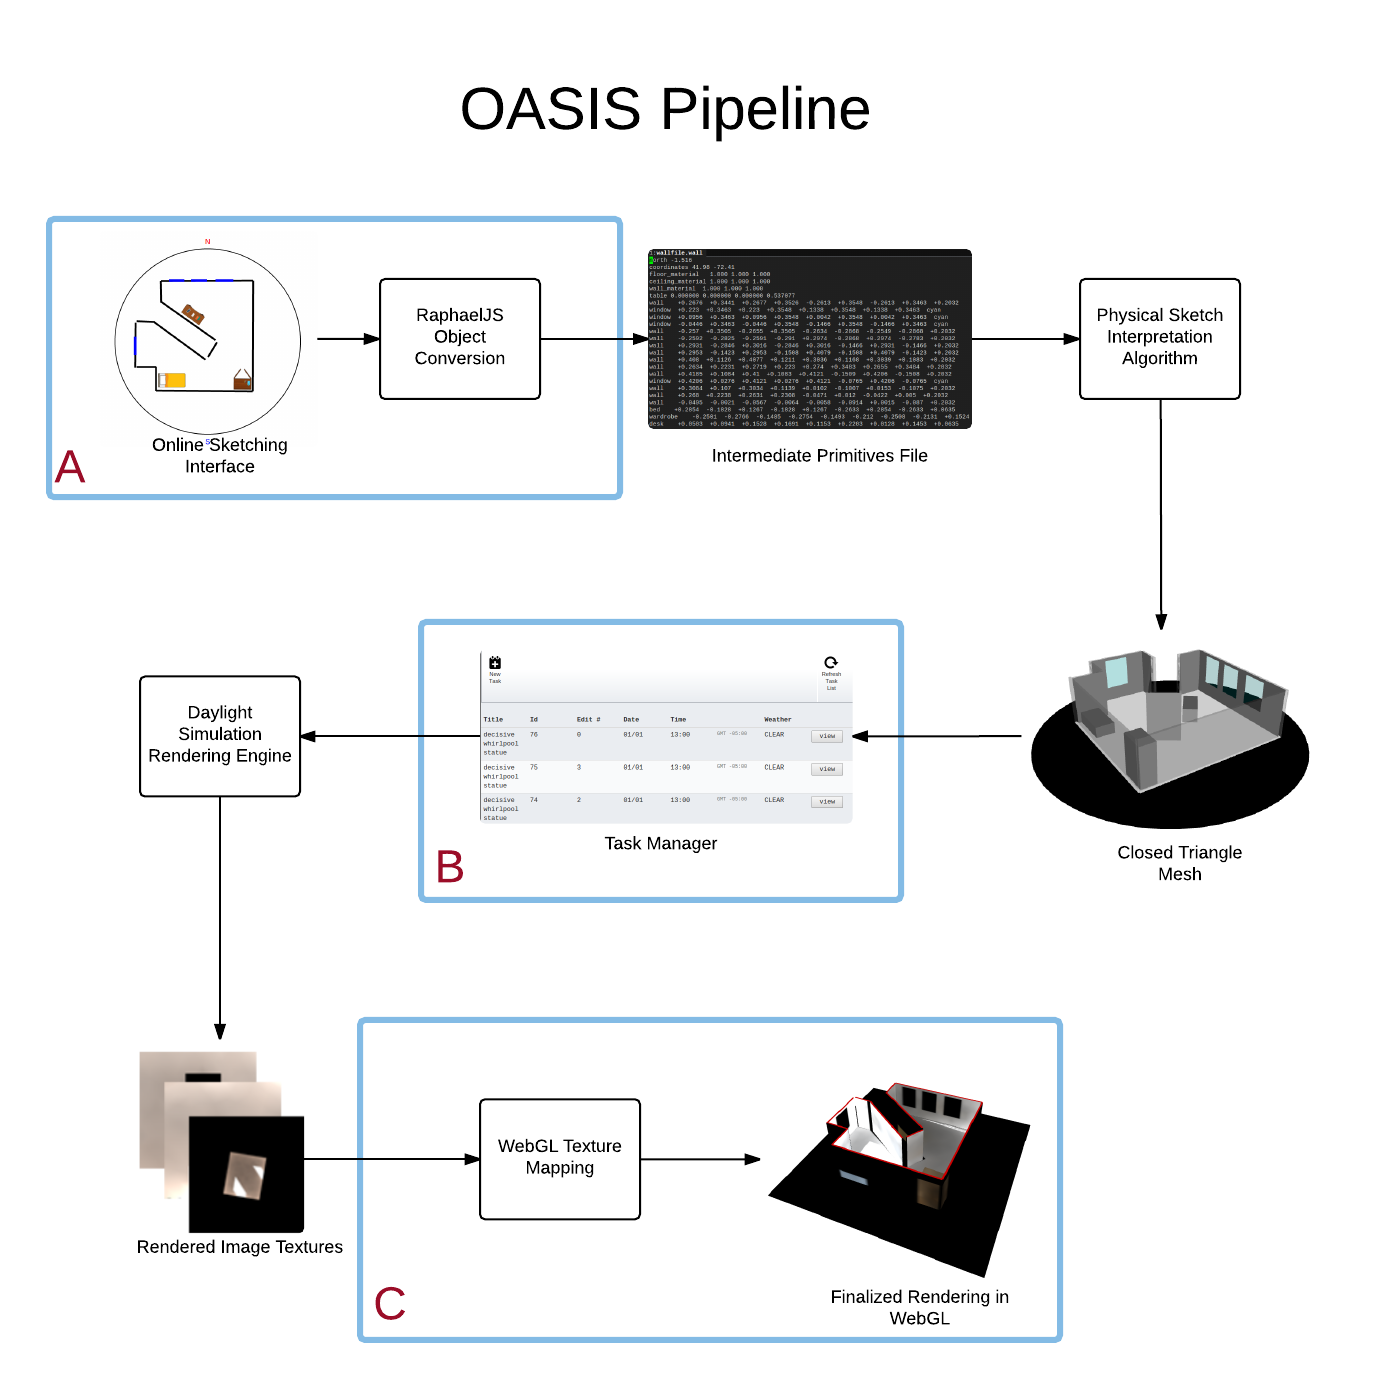
\includegraphics[width=15em]{img/new_pipeline.png}}\end{center}
The previous pipe line used a camera and image detection to create the primitive positions\cite{NasmanEvaluation, ShengYYC09 }, however with our online application we bypass image recognition and directly find the wall primitives and save those positions onto a database for later study. Those primitives go into the graphics pipeline and we get a triangle mesh model and rendered images with lighting textures, which are displayed on the screen as a 3D model. 
\vspace{1em}
    
      
   

  }

%%%%%%%%%%%%%%%%%%%%%%%%%%%%%%%%%%%%%%%%%%%%%%%%%%%%%%%%%%%%%%%%%%%%%%%%%%%%%%
\headerbox{Future Research}{name=future,column=2,row=1,below=userinterface,span = 2,bottomaligned=problem}{

\begin{multicols}{2}


	\textbf{Furniture Optimization}: A useful extension of the current pipeline that is under active research is furniture placement to maximize the utility of natural lighting. 
	Previous research \cite{NasmanEvaluation} offers us a way to visualize over and under illumination of a scene through false color textures. Future extensions of this would be intelligently select where to place common furniture items to maximize the use of natural daylighting. 
	Challenges faced are similar to previous work done on \emph{Make It Home}\cite{Yu} with the addition of quantifying daylighting usage. A clear set of challenges for implementing this feature is disccuesed blow:
	
	\begin{enumerate}\compresslist
   \item Relating illumination values given by the daylighting simulation real world measures.
   \item Creating a set of objects a spacial hierarchy of all objects modeled.
   \item Creation of a cost function based on\cite{Yu} with the addition of daylighting
   \item Choice of optimization the cost function to yield realistic results simulation
   \end{enumerate}
   
 \end{multicols}
 
 	
 \begin{center}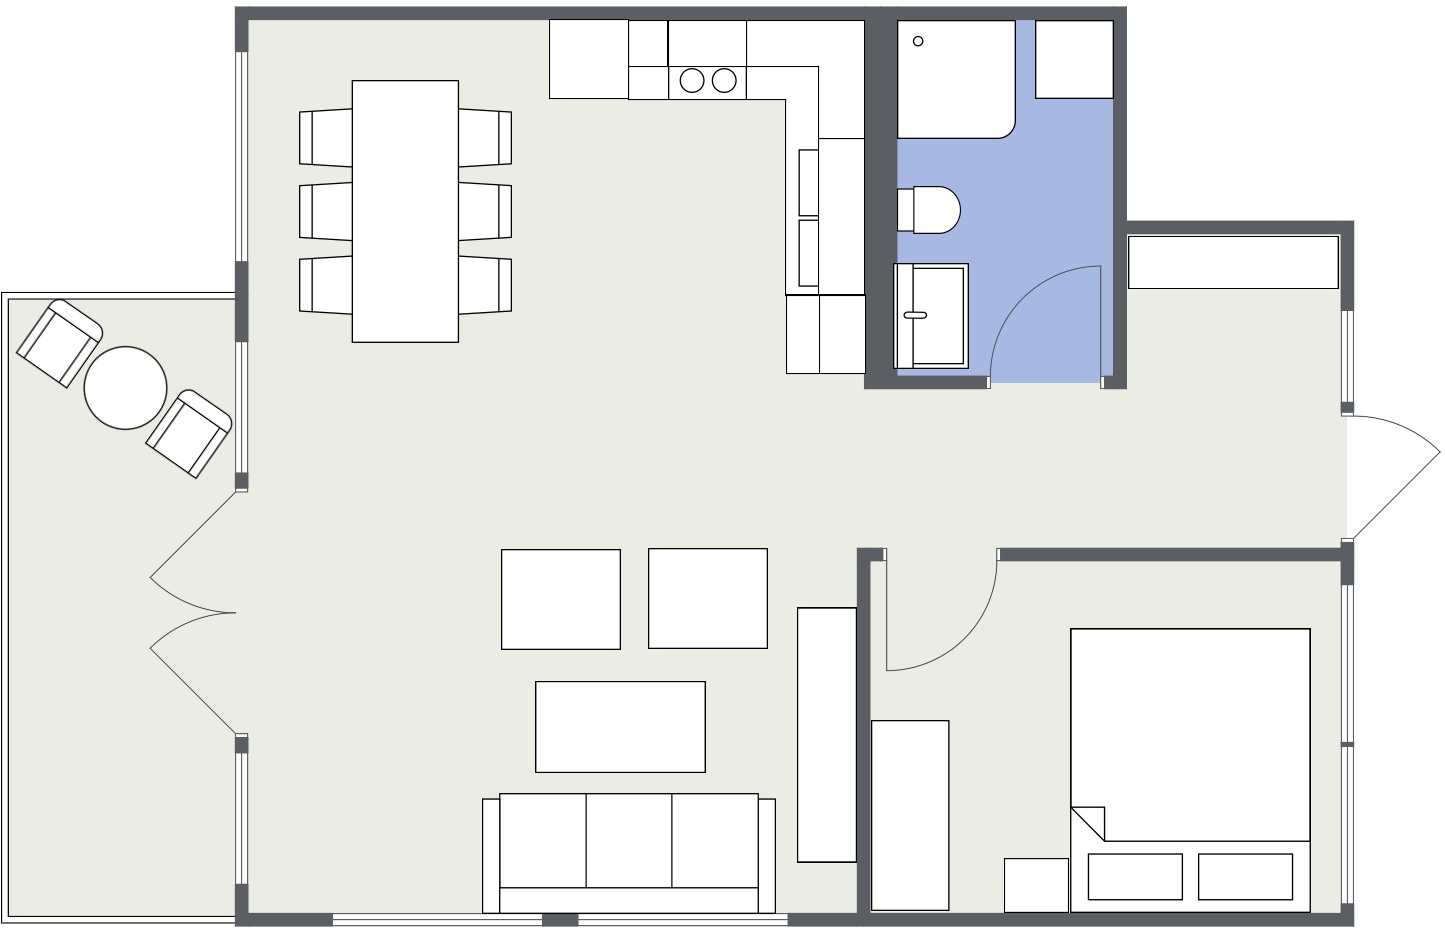
\includegraphics[height=6em]{img/layout.png}	 
 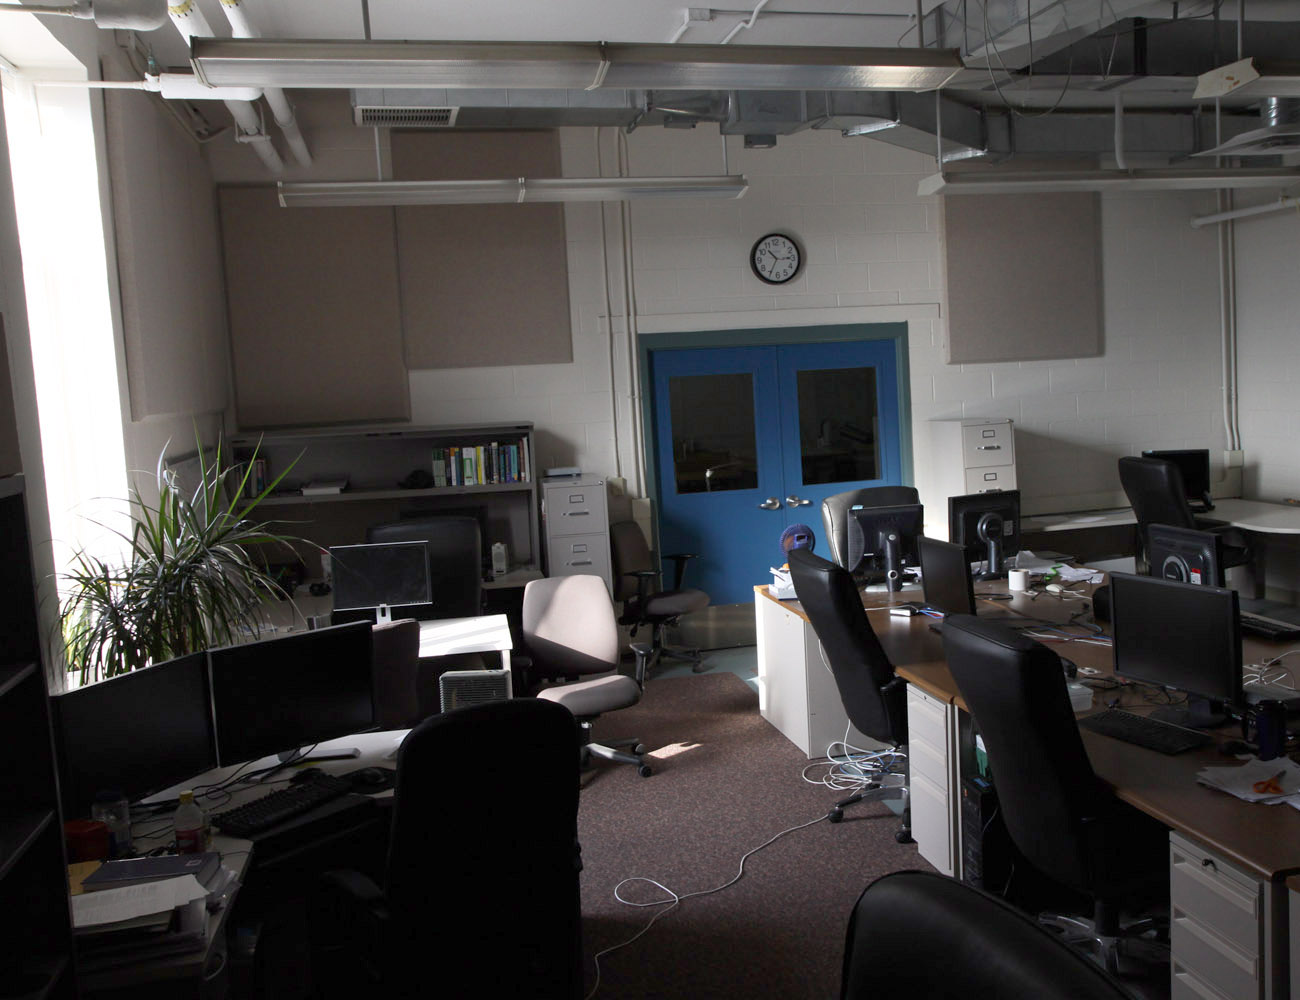
\includegraphics[height=6em]{img/room.jpg}	
 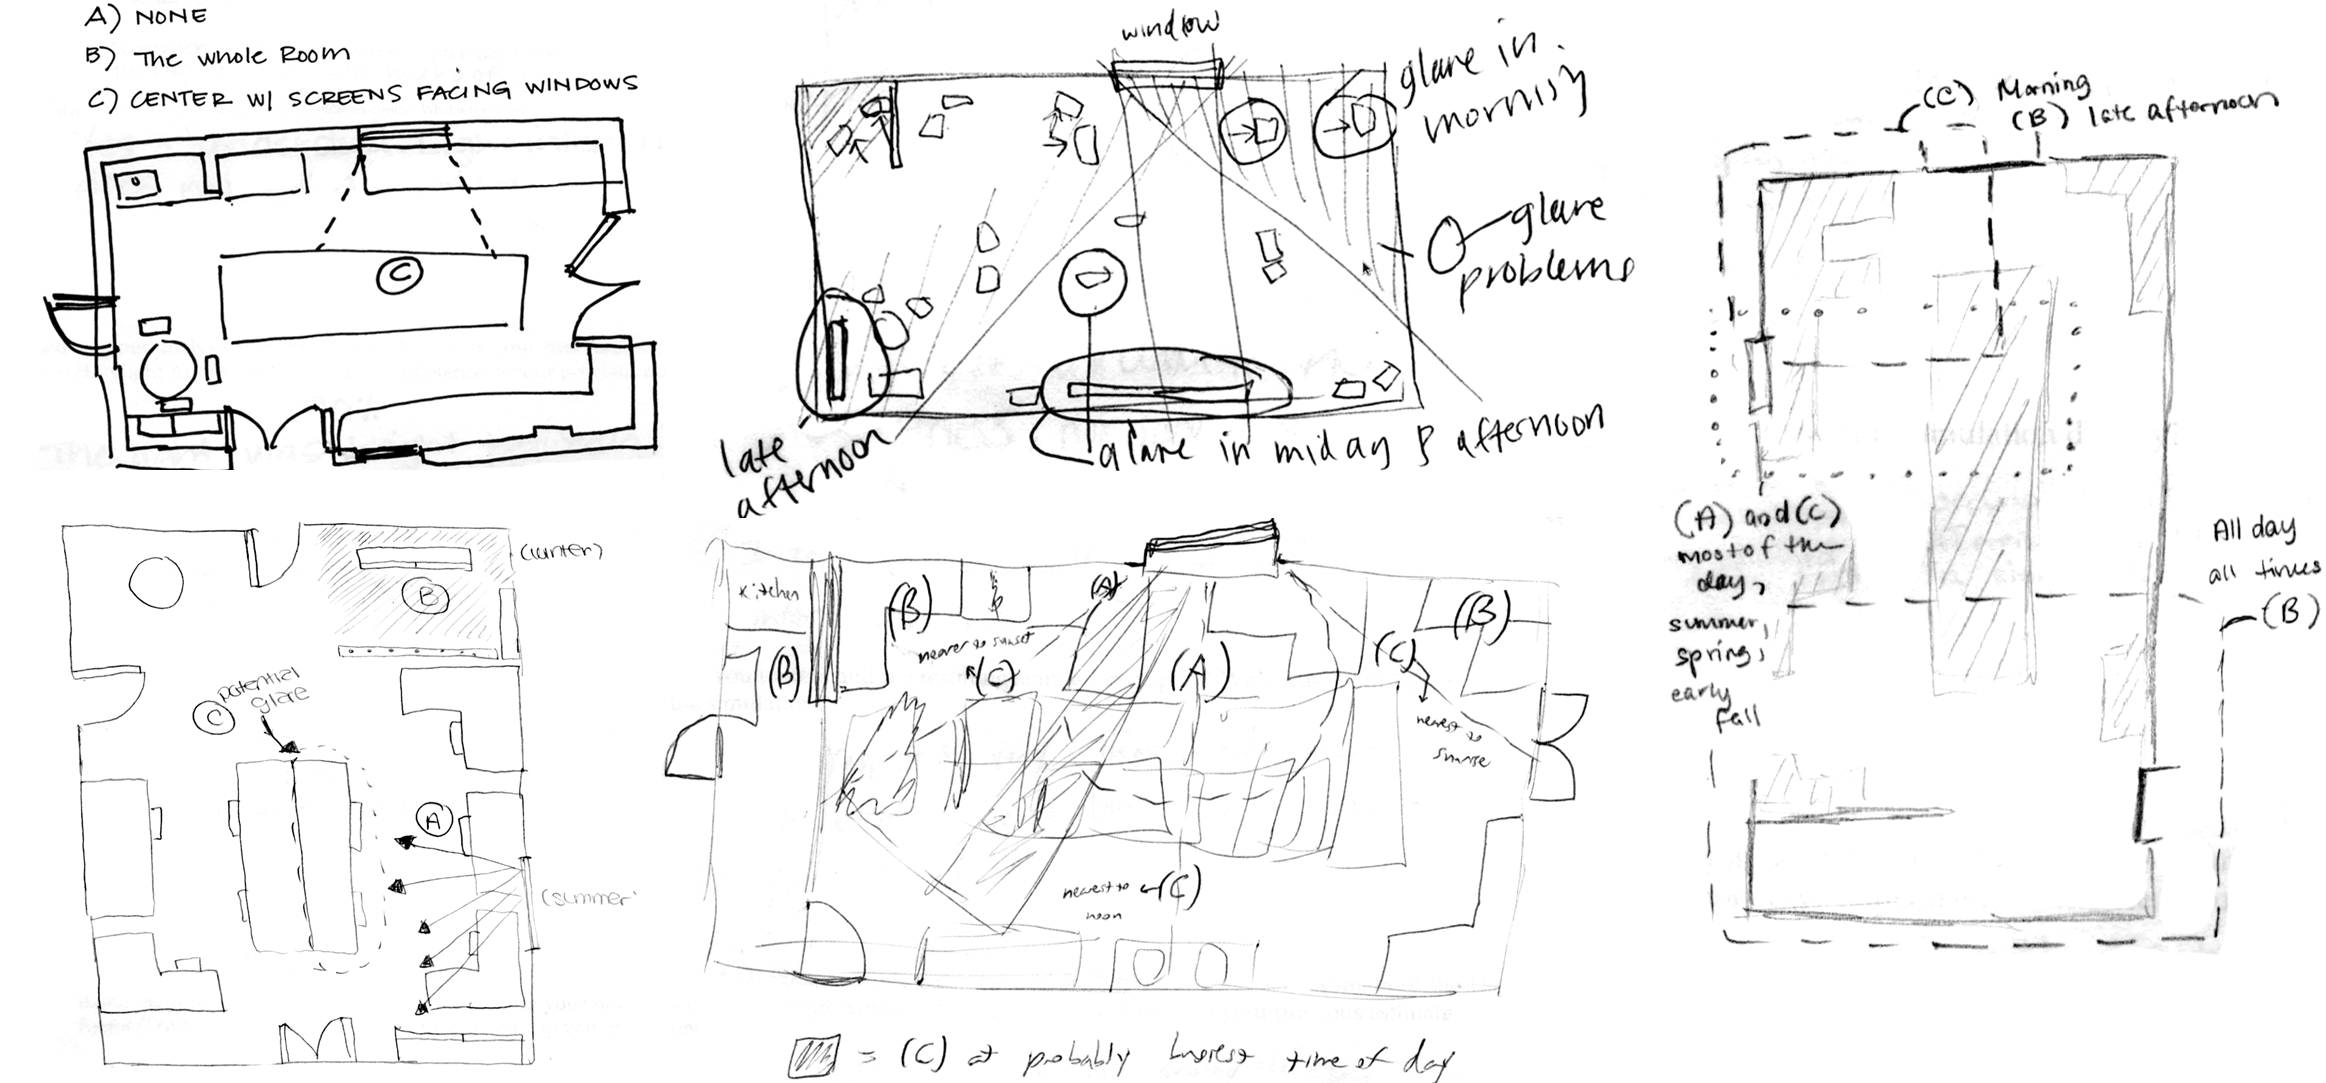
\includegraphics[height=6em]{img/all_together.png}	
  \end{center}
}
\headerbox{References}{name=credit, column = 1, row = 1, below = contribution, span = 1,bottomaligned=problem}{
{\tiny

\bibliography{cites}{}
\clearpage
\bibliographystyle{plain}

\par}
}

%%%%%%%%%%%%%%%%%%%%%%%%%%%%%%%%%%%%%%%%%%%%%%%%%%%%%%%%%%%%%%%%%%%%%%%%%%%%%
%%%%%%%%%%%%%%%%%%%%%%%%%%%%%%%%%%%%%%%%%%%%%%%%%%%%%%%%%%%%%%%%%%%%%%%%%%%%%%

\end{poster}
\end{document}












